\chapter{Axiomas de incidencia y orden}

%----------axioma 1
\begin{tcolorbox}[colframe=white]
    \begin{axioma}
	Cualquiera que sea la recta existen puntos que pertenecen a la recta y puntos que no pertenecen a la recta.
    \end{axioma}
\end{tcolorbox}

%----------axioma 2 
\begin{tcolorbox}[colframe=white]
    \begin{axioma}
	Dados dos puntos distintos existe una única recta que los contiene.
    \end{axioma}
\end{tcolorbox}

    %----------proposición 1.1.
    \begin{proposicion}
	Dos rectas distintas o no se intersectan o se intersectan en un único punto.\\\\
	    Demostración.-\; Sean $m,n$ dos rectas distintas, supongamos que $m,n$ se intersectan. Si $P,Q$ son puntos distintos donde $m,n$ se intersectan entonces por axioma 2, existe una única recta que contiene a $P$ y $Q$. Luego $m=n$ contrariamente a lo que supusimos a un principio, por lo tanto $P=Q$.\\\\
    \end{proposicion}

%----------axioma 3
\begin{tcolorbox}[colframe=white]
    \begin{axioma}
	Dados tres puntos de una recta, uno y sólo uno de ellos se localiza entre los otros dos.
    \end{axioma}
\end{tcolorbox}

%----------definición 1.1.
\begin{tcolorbox}[colframe=white]
    \begin{def.}[Segmento AB]
	Dados los puntos $A$ y $B$, el segmento $AB$ es el conjunto de puntos que están entre $A$ y $B$, y los puntos $A$ y $B$. Los puntos $A$ y $B$ se dicen extremos del segmento. Se denota con $\overline{AB}$.	
    \end{def.}
\end{tcolorbox}

%----------definición 1.2.
\begin{tcolorbox}[colframe=white]
    \begin{def.}
	Si $A$ y $B$ son puntos distintos, el conjunto que consiste en los puntos del segmento $AB$ y todos los puntos $C$ tales que $B$ está entre $A$ y $C$, se llama semi-recta de origen $A$ que contiene a $B$, y está representado por $S_{AB}$. El punto A se llama entonces el origen de la semi-recta $S_{AB}$.
    \end{def.}
\end{tcolorbox}

    %----------proposición 1.2
    \begin{proposicion}
	\begin{enumerate}[\bfseries a)]
	    \item $S_{AB} \cup S_{BA}$ es la recta $AB$\\\\
		Demostración.-\; Sea $m$ la recta $AB$, Es claro que $S_{AB} \subset m, \; S_{BA} \subset m;$ luego, $S_{AB} \cup S_{BA} \subset m$\\\\
	    \item $S_{AB} \cap S_{BA}= \overline{AB}$\\\\
		Demostración.-\; Por otro lado, si $C \in m$ entonces por axioma $3$, existen 3 posibilidades:
		\begin{enumerate}[1)]
		    \item $C$ está entre $A$ y $B$ entonces $C \in \overline{AB} \Rightarrow C\in S_{AB} \Rightarrow S\in S_{AB} \cup S_{BA}$.
		    \item $A$ está entre $C$ y $B$ entonces $C \in S_{BA} \Rightarrow C \in S_{AB} \cup S_{BA}$.
		    \item $B$ está entre $A$ y $C$ entonces $C \in S_{AB} \Rightarrow C \in S_{AB} \cup S_{BA}$.
		\end{enumerate}
	\end{enumerate}
	Por lo tanto, $m \subset S_{AB} \cup S_{BA}$. En conclusión de $1$ y $2$, $m=s_{AB} \cup S_{BA}$\\\\
    \end{proposicion}

%----------axioma 4
\begin{tcolorbox}[colframe=white]
    \begin{axioma}
	Dados dos puntos $A$ y $B$, siempre existen, un punto $C$ entre $A$ y $B$ y un punto $D$ tal que $B$ está entre $A$ y $D$.
    \end{axioma}
\end{tcolorbox}

%----------definición 1.3
\begin{tcolorbox}[colframe=white]
\begin{def.}
    Sea $m$ una recta y $A$ un punto tal que $A\notin m.$ El conjunto formado por los puntos de $m$ y por todos los puntos $B$ tales que $A$ y $B$ están en un mismo lado de la recta $m$ es llamado semi-plano determinado por $m$ y conteniendo a $A$.
\end{def.}
\end{tcolorbox}

%----------axioma 5 
\begin{tcolorbox}[colframe=white]
    \begin{axioma}
	Una recta $m$ determina exactamente dos semi-planos distintos cuya intersección es la recta $m$.
    \end{axioma}
\end{tcolorbox}

\section{Ejercicios}

\begin{enumerate}[\Large\bfseries 1.]

    %------------------1.
    \item Sobre una recta marque cuatro puntos $A,B,C$ y $D$ en orden, de izquierda a derecha. Determine:\\

	    \begin{center}
	    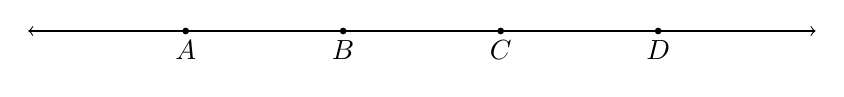
\begin{tikzpicture}
		\draw[<->] (0,0)--(10,0);
		\filldraw[black] (2,0) circle (1pt) node[below]{$A$};
		\filldraw[black] (4,0) circle (1pt) node[below]{$B$};
		\filldraw[black] (6,0) circle (1pt) node[below]{$C$};
		\filldraw[black] (8,0) circle (1pt) node[below]{$D$};
	    \end{tikzpicture}
	    \end{center}

	\begin{enumerate}[\bfseries (a)]
	\begin{multicols}{2}

	    %----------(a)
	    \item $AB \cup BC$\\\\
	    Respuesta.-\; AC\\\\

	    %----------(b)
	    \item $AB \cap BC$\\\\
	    Respuesta.-\; B \\\\

	    %----------(c)
	    \item $AC \cap BD$\\\\
	    Respuesta.-\; BC\\\\

	    %----------(d)
	    \item $AB \cap CD$\\\\ 
	    Respuesta.-\; $\empty$\\\\

	    %----------(e)
	    \item $S_{AB} \cap S_{BC}$\\\\
	    Respuesta.-\; $S_{BC}$ \\\\

	    %----------(f)
	    \item $S_{AB} \cap S_{AD}$\\\\
	    Respuesta.-\; $S_{AB}$\\\\

	    %----------(g)
	    \item $S_{CB} \cap S_{BC}$\\\\
	    Respuesta.-\; BC \\\\

	    %----------(h)
	    \item $S_{AB} \cup S_{BC}$\\\\
	    Respuesta.-\; $S_{AB}$\\\\
	\end{multicols}
	\end{enumerate}

    %--------------------2.
    \item Pruebe que en un segmento existen infinitos puntos.\\\\
    Demostración.-\; Sea una recta $m$ con puntos distintos $A$ y $B$, supongamos que entre $A$ y $B$ hay puntos finitos, entonces por definición un conjunto es finito cuando puede ser colocado en correspondencia biunívoca en un conjunto $\mathbb{N}$. Luego $AB$ es un conjunto con $n$ elementos $AB=\lbrace P_1,P_2,...,P_n \rbrace$\\\\

    %--------------------3.
    \item Sean $P=\lbrace a,b,c \rbrace$, $m_1=\lbrace a,b \rbrace$, $m_2=\lbrace a,c \rbrace$ y $m_3=\lbrace b,c \rbrace$. Llame a $P$ el plano y a $m_1,m_2$ y $m_3$ rectas. Verifique en esta $"$geometría$"$ si es cierto el axioma $I_2$.\\\\
    Demostración.-\; Observemos que todas las combinaciones posibles entre los puntos del plano $P$, tomadas de dos en dos pertenecen a una de las tres líneas rectas de esa geometría. Es decir $ab,ac,ba,bc,ca,cb$. Debemos fijarnos que solo la línea $m_1$ pasa por $ab$. Del mismo modo para los otros pares de puntos, pasan sólo una de las líneas mencionadas $m_1,m_2,m_3$. Esto muestra que en ésta geometría vale el axioma $I_2$\\\\

    %--------------------4.
    \item Un subconjunto del plano se dice convexo si el segmento que une dos puntos cualesquiera de sus puntos está totalmente contenido en él. Los ejemplos más simples de conjuntos convexos son el propio plano y cualquier semiplano. Muestre que la intersección de dos semiplanos es un conjunto convexo.\\\\
    Demostración.-\; Supongamos los semiplanos $S_1,S_2$ y $S_3$ tal que $S_3 = S_1 \cap S_2$ tomando dos puntos $A, B \in S_3$ entonces: $$A,B \in S_1,S_2$$ Sean $S_1$ y $S_2$ convexos entonces $A,B \in S_1,S_2$ y por lo tanto pertenecen  a la intersección, luego $S_3$ es convexo.\\\\


    %--------------------5.
    \item Muestre, dando un contraejemplo, que la unión de convexos puede no ser un conjunto convexo.\\\\
    Demostración.-\; Los cuatro rectángulos en gris son figuras convexas y su unión forma una figura con una cavidad, parte en blanco y por lo tanto cóncava.
    \begin{center}
	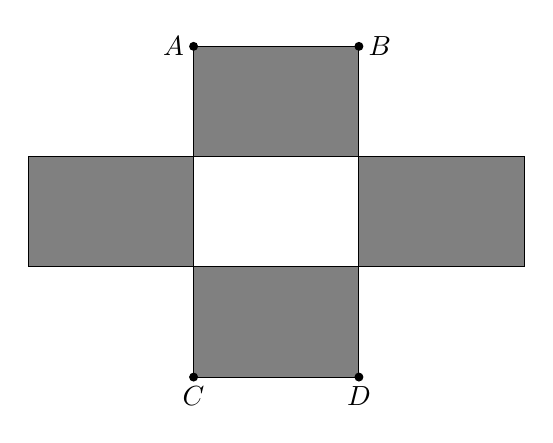
\begin{tikzpicture}[scale=.7]
	    \draw[fill=gray](0,0) rectangle (3,2);
	    \draw[fill=gray](3,-2) rectangle (6,0);
	    \draw[fill=gray](0,-4) rectangle (3,-2);
	    \draw[fill=gray](-3,-2) rectangle (0,0);
	    \filldraw[black](0,2) circle(2pt) node[left]{$A$};
	    \filldraw[black](3,2) circle(2pt) node[right]{$B$};
	    \filldraw[black](0,-4) circle(2pt) node[below]{$C$};
	    \filldraw[black](3,-4) circle(2pt) node[below]{$D$};
	\end{tikzpicture}
    \end{center}

    %--------------------6.
    \item Tres puntos no colineales determinan tres rectas. ¿Cuántas rectas son determinadas por cuatro puntos tal que cualesquier tres de ellos no son colineales.?\\\\
    Respuesta.-\; Veamos la siguiente tabla, donde $r_{ij}$ y la linea determinada por los puntos $P_i$ y $P_j$
    \begin{center}
	\begin{tabular}{cccc}
	    &$P_1$&$P_2$&$P_3$\\
	    $P_1$&$-$&$r_{12}$&$r_{13}$\\
	    $P_2$&$r_{21}$&$-$&$r_{23}$\\
	    $P_3$&$r_{31}$&$r_{32}$&$-$\\
	\end{tabular}
    \end{center}
    El número de líneas será $\dfrac{3(3-1)}{2}=3$ y por $n$ puntos $\dfrac{n(n-1)}{2}$\\\\

    %--------------------7.
    \item Repita el ejercicio anterior para el caso de $6$ puntos.\\\\
    Respuesta.-\; $\dfrac{6(6-1)}{2}=15$\\\\

    %--------------------8.
    \item Pruebe que, si una recta interseca un lado de un triángulo y no pasa por ninguno de sus vértices, entonces ella intersecta también uno de los otros dos lados.\\\\
    Demostración.-\; Dado un triángulo $ABC$ y una recta $m$, si $m$ interseca el segemento $AB$, entonces $A$ está en el lado puesto de $B$ con respecto a la recta $m$. Como por hipótesis $m$ no pasa por $C$, entonces $C$ está del lado de $A$ ó $B$.\\
    Si $C$ está del lado de $A$, entonces $C$ es opuesto a $B$ y luego $m$ interseca a $BC$.\\
    Si $C$ está del lado de $B$, entonces es contrario a $A$ y $m$ interceca $AC$.\\
    Entonces siempre interseca un lado.\\\\

    %--------------------9.
    \item Muestre que no existe una $"$geometría$"$ con $6$ puntos, donde sean válidos los axiomas $I_1$ y $I_2$ y que todas las rectas tengan exactamente $3$ puntos.\\\\   
    Demostración.-\; Sea una recta $m=\lbrace P_1,P_2 \rbrace$ por hipótesis existe un $Q_1 \in P$ diferente de $P_1$ y $P_2$.\\
    Luego sea $Q_2 \in P$ y diferente de $P_1,P_2$ y $Q_1$, por hipótesis, tenemos que $Q_2 \notin m$ porque $m$ ya tiene 3 puntos. Por tanto, hay una línea recta $n=\lbrace P_1,Q_2 \rbrace$ y que contiene un punto $Q_3\in P$ con $Q_3\neq P_1,P_2,Q_1,Q_2$\\
    Ahora tome $Q_4 \in P$ con $Q_4 \neq P_1,P_2,Q_1, Q_2,Q_3$. Nuevamente por hipótesis $Q_4 \notin m,n$ porque ambos ya tienen tres puntos. Entonces debe haber una línea $t=\lbrace P_1,Q_4 \rbrace$ que debe contener por hipótesis, un tercer punto $Q5$. Entonces tenemos $Q_5 \neq P_1$ y $Q_5 \neq Q_4$, luego $Q_5 \neq Q_1$ y $Q_5\neq P_2$ porque $m\neq t$, $Q_5\neq Q_2$ y $Q_5\neq Q_3$ ya que $n\neq t$. Esto nos lleva a una contradicción porque $Q_5$ sería el séptimo punto de la geometría dada.\\\\

    %--------------------10.
    \item Si $C$ pertenece a $S_{AB}$ y $C\neq A,$ muestre que: $S_{AB}=S_{AC}, BC \subset S_{AB}$ y que $A \notin BC.$\\\\
    Demostración-.\; Dada una semirecta $S_{AB}$ a través de los puntos $A$ y $B$ determinamos la semirrecta $S_{BA}$ donde por la proposición $S_{AB} \cup S_{BA}$ esta contenido en la recta $m$. Luego por definición $S_{AB}$  es el conjunto de puntos en el segmento $AB$ más el conjunto de puntos $X$ tales que $A-B-X$.\\
    Como $C\in S_{AB}$ por hipótesis ocurre una de las tres posibilidades:
    \begin{enumerate}[\bfseries 1.]
	\item $C=B$ en este caso la demostración es trivial.
	\item $A-B-C$ En este caso, por definición de semi-recta $S_{AB}=S_{AC}$ siendo $BC=S:{bC} \cap S_{CA}$ y como $A\notin S_{BC}$ entonces $A\notin BC$.
	\item $A-C-B$ se demuestra análogamente al caso anterior.\\\\
    \end{enumerate}

    %--------------------11.
    \item Muestre que un triángulo separa el plano en dos regiones, una de las cuales es convexa.\\\\
    Demostración.-\; Tracemos tres rectas $m,n$ y $o$ que se intersecan en los puntos $A,B$ y $C$ de la manera siguiente:
    \begin{center}
	\begin{tikzpicture}[scale=0.5]
	    \draw[<->](-2,0)--(12,0)node[above]{$n$};
	    \draw[<->](-1,-2)--(6,6)node[right]{$o$};
	    \draw[<->](10,-2)--(4,6)node[left]{$m$};
	    \filldraw[black](.8,0) circle(2pt) node[below right]{$C$};
	    \filldraw[black](8.5,0) circle(2pt) node[below left]{$B$};
	    \filldraw[black](4.9,4.8) circle(2pt) node[right]{$A$};
	    \filldraw[black](5.2,2.6) circle(2pt) node[below]{$X$};
	    \filldraw[black](3,1.3) circle(2pt) node[below]{$Y$};
	    \filldraw[black](4.9,4.2) node[below]{$\alpha$};
	\end{tikzpicture}
    \end{center}
    Así formamos el triángulo $ABC$, que a su vez separa el plano en dos regiones. La región convexa es la región que forma el interior del triángulo. Para probar esto, considere los puntos $X$ e $Y$ que pertenecen al semiplano llamemosle $\alpha$ generado por las tres rectas. Dado que $X$ e $Y$ están en el mismo semiplano generado por la recta $m$, entonces el segmento $XY$ no interseca a la recta $m$. De manera similar, $XY$ no puede interceptar las líneas $n$ y $o$. Esto implica que $XY$ pertenece al semiplano $\alpha$ formado por el triángulo $ABC$, que por tanto es una región convexa.\\\\

    %--------------------12.
    \item ¿Puede existir dos segmentos distintos con dos puntos en común?¿Y, teniendo exactamente dos puntos en común?\\\\
    Respuesta.-\; Dados los puntos $A, B, C$ y $D$ de modo que $ABCD$ entonces los segmentos $AC$ y $BD$ tendrán el segmento $BC$ en común ya que en un segmento hay puntos infinitos por lo que $AC$ y $BD$ tienen dos puntos en común pero nunca solo tendrán dos puntos.\\\\

\end{enumerate}

